%------------------------------------------------------------------------------
% CV
% Hafez Ghaeemi
%------------------------------------------------------------------------------

\documentclass[A4,11pt]{article}
%\documentclass[letterpaper,11pt]{article} %For use in US
\usepackage{latexsym}
\usepackage[empty]{fullpage}
\usepackage{titlesec}
\usepackage{marvosym}
\usepackage{tabto}
\usepackage[usenames,dvipsnames]{color}
\usepackage{verbatim}
\usepackage{enumitem}
\usepackage[hidelinks]{hyperref}
\usepackage[english]{babel}
\usepackage{tabularx}
\usepackage{tikz}
%\input{glyphtounicode}

% serif
 \usepackage{palatino}
% \usepackage{times} %This is the default as well
% \usepackage{charter}

% sans-serif
% \usepackage{helvet}
% \usepackage[sfdefault]{noto-sans}
% \usepackage[default]{sourcesanspro}

%-----PAGE SETUP---------------------------------------------------------------

% Adjust margins
\addtolength{\oddsidemargin}{-1cm}
\addtolength{\evensidemargin}{-1cm}
\addtolength{\textwidth}{2cm}
\addtolength{\topmargin}{-1cm}
\addtolength{\textheight}{2cm}

% Margins for US Letter size
%\addtolength{\oddsidemargin}{-0.5in}
%\addtolength{\evensidemargin}{-0.5in}
%\addtolength{\textwidth}{1in}
%\addtolength{\topmargin}{-.5in}
%\addtolength{\textheight}{1.0in}

\urlstyle{same}

\raggedbottom
\raggedright
\setlength{\tabcolsep}{0cm}

% Sections formatting
\titleformat{\section}{
  \vspace{-4pt}\scshape\raggedright\large
}{}{0em}{}[\color{black}\titlerule \vspace{-5pt}]

% Ensure that .pdf is machine readable/ATS parsable
%\pdfgentounicode=1

%-----CUSTOM COMMANDS FOR FORMATTING SECTIONS----------------------------------
\newcommand{\CVItem}[1]{
  \item\small{
    {#1 \vspace{-2pt}}
  }
}

\newcommand{\CVSubheading}[4]{
  \vspace{-2pt}\item
    \begin{tabular*}{0.97\textwidth}[t]{l@{\extracolsep{\fill}}r}
      \textbf{#1} & #2 \\
      \small#3 & \small #4 \\
    \end{tabular*}\vspace{-7pt}
}

\newcommand{\CVSubSubheading}[2]{
    \item
    \begin{tabular*}{0.97\textwidth}{l@{\extracolsep{\fill}}r}
      \text{\small#1} & \text{\small #2} \\
    \end{tabular*}\vspace{-7pt}
}

\newcommand{\CVSubItem}[1]{\CVItem{#1}\vspace{-4pt}}

\renewcommand\labelitemii{$\vcenter{\hbox{\tiny$\bullet$}}$}

\newcommand{\CVSubHeadingListStart}{\begin{itemize}[leftmargin=0.5cm, label={}]}
% \newcommand{\resumeSubHeadingListStart}{\begin{itemize}[leftmargin=0.15in, label={}]} % Uncomment for US
\newcommand{\CVSubHeadingListEnd}{\end{itemize}}
\newcommand{\CVItemListStart}{\begin{itemize}}
\newcommand{\CVItemListEnd}{\end{itemize}\vspace{-5pt}}

\usepackage{etoolbox,refcount}
\usepackage{multicol}

\newcounter{countitems}
\newcounter{nextitemizecount}
\newcommand{\setupcountitems}{%
  \stepcounter{nextitemizecount}%
  \setcounter{countitems}{0}%
  \preto\item{\stepcounter{countitems}}%
}
\makeatletter
\newcommand{\computecountitems}{%
  \edef\@currentlabel{\number\c@countitems}%
  \label{countitems@\number\numexpr\value{nextitemizecount}-1\relax}%
}
\newcommand{\nextitemizecount}{%
  \getrefnumber{countitems@\number\c@nextitemizecount}%
}
\newcommand{\previtemizecount}{%
  \getrefnumber{countitems@\number\numexpr\value{nextitemizecount}-1\relax}%
}
\makeatother    
\newenvironment{AutoMultiColItemize}{%
\ifnumcomp{\nextitemizecount}{>}{3}{\begin{multicols}{2}}{}%
\setupcountitems\begin{itemize}}%
{\end{itemize}%
\unskip\computecountitems\ifnumcomp{\previtemizecount}{>}{3}{\end{multicols}}{}}


%------------------------------------------------------------------------------
% CV STARTS HERE  %
%------------------------------------------------------------------------------
\begin{document}

%-----HEADING------------------------------------------------------------------
%
%\begin{minipage}[c]{0.05\textwidth}
%\-\
%\end{minipage}
%%\begin{minipage}[c]{0.2\textwidth}
%%\begin{tikzpicture}
%%    \clip (0,0) circle (1.75cm);
%%    \node at (-0.3,1.6) {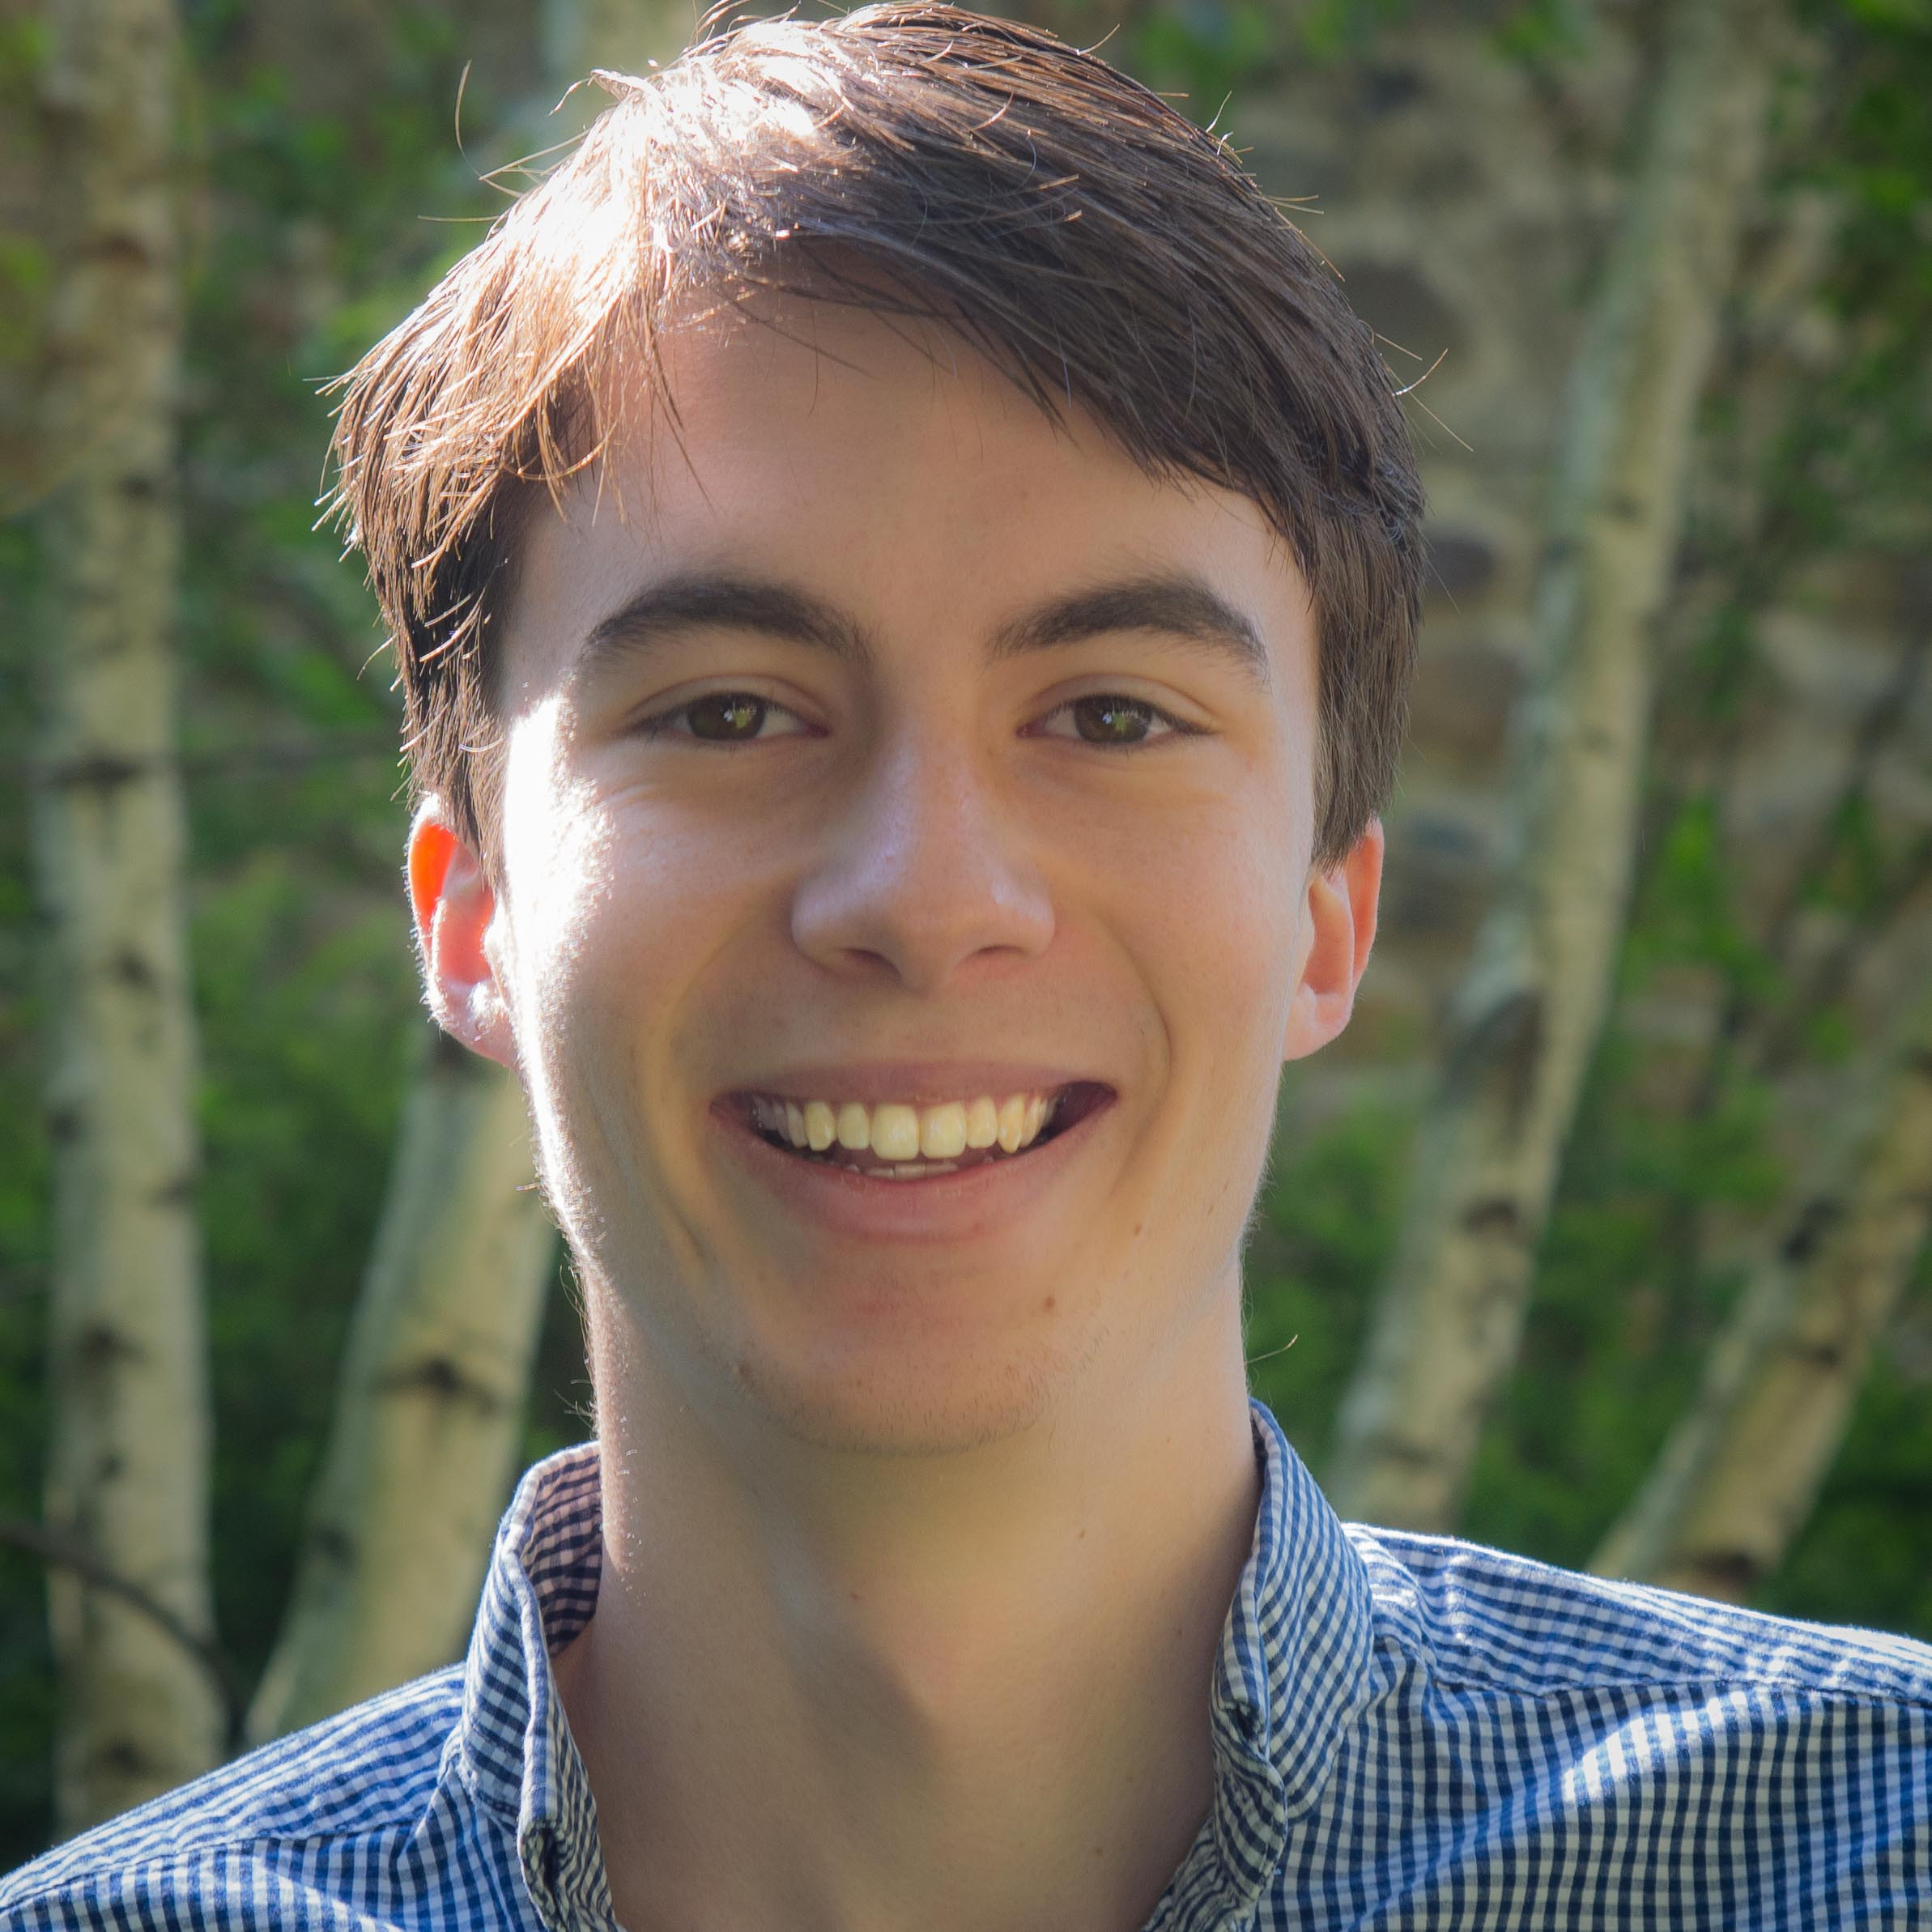
\includegraphics[width = 10cm]{portrait}}; 
%%    % if necessary the picture may be moved by changing the at (coordinates)
%%    % width defines the 'zoom' of the picture
%%\end{tikzpicture}
%\hfill\vline\hfill
%\end{minipage}
\begin{minipage}[c]{0.4\textwidth}
    \textbf{\Huge \scshape{Hafez Ghaemi}} \href{https://orcid.org/0000-0001-6326-5258}{
\includegraphics[width=0.07\textwidth]{orcid}} \\ \vspace{1pt} 
    % \scshape sets small capital letters, remove if desired
    \href{mailto:hafez.ghaemi@umontreal.ca}{\underline{hafez.ghaemi@umontreal.ca}}\\ \vspace{1pt} 
      \href{https://hafezgh.github.io/}{\underline{hafezgh.github.io}}\\ \vspace{1pt} 
      \href{https://mila.quebec/en/person/hafez-ghaemi/}{\underline{mila.quebec/en/person/hafez-ghaemi/}} \\ \\  \vspace{1pt}
   % \href{mailto:hafez.ghaemi@mila.quebec}{\underline{hafez.ghaemi@mila.quebec}}\\
    % Be sure to use a professional *personal* email address
    % you should adjust you linked in profile name to be professional and recognizable
    \href{https://scholar.google.com/citations?user=JCLX6oYAAAAJ&hl=en}{
\includegraphics[width=0.1\textwidth]{scholar}}
    \href{https://github.com/hafezgh}{
\includegraphics[width=0.1\textwidth]{github}}
    \href{https://www.linkedin.com/in/hafez-ghaemi-618b8287/}{
\includegraphics[width=0.1\textwidth]{linkedin}}
    \href{https://x.com/hafezghm}{
\includegraphics[width=0.1\textwidth]{x}}\\
    Last updated: July 15, 2024
\end{minipage}

% Without picture
%\begin{center}
%    \textbf{\Huge \scshape Charles Rambo} \\ \vspace{1pt} %\scshape sets small capital letters, remove if desired
%    \small +1 123-456-7890 $|$ 
%    \href{mailto:you@provider.com}{\underline{you@provider.com}} $|$\\
%    % Be sure to use a professional *personal* email address
%    \href{https://linkedin.com/in/your-name-here}{\underline{linkedin.com/in/charles-rambo}} $|$
%    % you should adjust you linked in profile name to be professional and recognizable
%    \href{https://github.com/fizixmastr}{\underline{github.com/fizixmastr}}
%\end{center}

\section{Education}
  \CVSubHeadingListStart
%    \CVSubheading % Example
%      {Degree Achieved}{Years of Study}
%      {Institution of Study}{Where it is located}
    \CVSubheading
      {{Ph.D. $|$ \emph{Computer Science}}}{Aug. 2023 -- Present}
      {\href{https://mila.quebec/en/}{\underline{Mila}} - \href{https://diro.umontreal.ca/english/home/}{\underline{University of Montreal}}; \textbf{GPA:} 4.13/4.0}{Montreal, QC, Canada}
      \CVItemListStart
        \CVItem{\textbf{Advisors}: \href{https://scholar.google.ch/citations?user=r4-NZhwAAAAJ&hl=en}{\underline{Eilif Muller}},
        \href{https://scholar.google.com/citations?user=f_JDOhEAAAAJ&hl=en}{\underline{Shahab Bakhtiari}}; \textbf{Doctoral Committee:} \href{https://scholar.google.com/citations?hl=en&user=km6CP8cAAAAJ&view_op=list_works}{\underline{Aaron Courville}},
        \href{https://scholar.google.com/citations?hl=en&user=WBCKQMsAAAAJ&view_op=list_works}{\underline{Pascal Vincent}}}
      \CVItemListEnd
    \CVSubheading
      {{M.Sc. $|$ \emph{Computer Engineering, AI and Robotics}}}{Sep. 2020 -- Aug. 2023}
      {\href{https://ut.ac.ir/en}{\underline{University of Tehran}}; \textbf{GPA:} 18.0/20.0, North American: 3.72/4.0}{Tehran, Iran}
      \CVItemListStart
        \CVItem{\textbf{Advisors}: \href{https://scholar.google.com/citations?user=eDseLNYAAAAJ&hl=en}{\underline{Hamed Kebriaei}},
        \href{https://scholar.google.com/citations?user=QlwWxmoAAAAJ&hl=en}{\underline{Majid Nili}}; \textbf{Thesis}: Cumulative Prospect Theory in Multi-Agent Reinforcement Learning and Markov Games
        	(\href{https://arxiv.org/abs/2402.05906}{\underline{paper}}) (\href{https://github.com/hafezgh/risk-sensitive-marl-namg}{\underline{code}})}
      \CVItemListEnd
    \CVSubheading
      {{M.Sc. $|$ \emph{\small{Data Science and Engineering}}}}{Sep. 2020 -- July 2022}
      {\href{https://www.polito.it/en?lang=en}{\underline{Politecnico di Torino}}; \textbf{GPA:} 26.3/30.0 (103/110), North American: 3.7/4.0}{Turin, Italy}
      \CVItemListStart
        \CVItem{\textbf{Advisors}: \href{https://scholar.google.com/citations?user=oqwlDQEAAAAJ&hl=en}{\underline{Fabio Fagnani}},
        \href{https://scholar.google.com/citations?user=7dju3QoAAAAJ&hl=en}{\underline{Giacomo Como}}; \textbf{Thesis}: Decentralized Value-Based Reinforcement Learning in Stochastic Potential Games (\href{https://webthesis.biblio.polito.it/23450/}{\underline{link}}) (\href{https://github.com/hafezgh/PoliTo-MSc-Thesis}{\underline{code}})}
      \CVItemListEnd
    \CVSubheading
      {{B.Sc. $|$ \emph{\small{Major: Mechanical Engineering, Minor: Computer Engineering}}}}{Sep. 2016 -- Sep. 2020}
      {{University of Tehran}; \textbf{GPA:} 16.24/20.0, North American: 3.35/4.0}{Tehran, Iran}
    \CVItemListStart
        \CVItem{\textbf{Advisor}: \href{https://scholar.google.com/citations?user=UwlyBw0AAAAJ&hl=en}{\underline{Masoud Shariat Panahi}}; \textbf{Thesis}: Design and Implementation of A Smart Camera Slider Controller with Deep Reinforcement Learning (\href{https://github.com/hafezgh/bahcelor_thesis}{\underline{code}})}
    \CVItemListEnd
  \CVSubHeadingListEnd

%-----WORK EXPERIENCE----------------------------------------------------------

\section{Publications}
%    \CVSubheading %Example
%      {What you did}{When you worked there}
%      {Who you worked for}{Where they are located}
%      \CVItemListStart
%        \CVItem{Why it is important to this employer}
%      \CVItemListEnd
\CVItemListStart
\CVItem{\textbf{H. Ghaemi}, H. Kebriaei, A. R. Moghaddam, and M. Nili Ahamdabadi. "Risk-Sensitive Multi-Agent Reinforcement Learning in Network Aggregative Markov Games", Proceedings of the 23rd International Conference on Autonomous Agents and Multiagent Systems, 2024. (\href{https://dl.acm.org/doi/10.5555/3635637.3663134}{\underline{link}}), (\href{https://arxiv.org/abs/2402.05906}{\underline{preprint}}), (\href{https://github.com/hafezgh/risk-sensitive-marl-namg/blob/main/Poster_RSMARL_AAMAS2024.pdf}{\underline{poster}}) (\href{https://github.com/hafezgh/risk-sensitive-marl-namg/}{\underline{code}})}

\CVItem{M. Nouri*, F. Moradi*, \textbf{H. Ghaemi}*, A. M. Nasrabadi, "Towards real-world BCI: CCSPNet, a compact subject-independent motor imagery framework", Digital Signal Processing, 2023. *: equal contribution. (\href{https://doi.org/10.1016/j.dsp.2022.103816}{\underline{link}}), (\href{https://arxiv.org/abs/2012.13567}{\underline{preprint}}), (\href{https://github.com/Singular-Brain/CCSPNet}{\underline{code}})}

\CVItem{\textbf{H. Ghaemi}*, E. Mirzaei*, M. Nouri*, and S. R. Kheradpisheh "BioLCNet: Reward-modulated Locally Connected Spiking Neural Networks", International Conference on Machine Learning, Optimization, and Data Science, 2022. *: equal contribution. (\href{https://doi.org/10.1007/978-3-031-25891-6_42}{\underline{link}}), (\href{https://arxiv.org/abs/2109.05539}{\underline{preprint}}) (\href{https://github.com/Singular-Brain/BioLCNet}{\underline{code}})}


\CVItemListEnd


%\section{In Press}
%    \CVSubheading %Example
%      {What you did}{When you worked there}
%      {Who you worked for}{Where they are located}
%      \CVItemListStart
%        \CVItem{Why it is important to this employer}
%      \CVItemListEnd
%\CVItemListStart
%\CVItem{\textbf{Hafez Ghaemi}, Hamed Kebriaei, Alireza Ramezani Moghaddam, and Majid Nili Ahamdabadi. "Risk-Sensitive Multi-Agent Reinforcement Learning in Network Aggregative Markov Games." (To be presented in AAMAS 2024 Conference), (\href{https://arxiv.org/abs/2402.05906}{\underline{preprint}}), (\href{https://github.com/hafezgh/risk-sensitive-marl-namg}{\underline{code})}}
%\CVItemListEnd



\section{Preprints}
%    \CVSubheading %Example
%      {What you did}{When you worked there}
%      {Who you worked for}{Where they are located}
%      \CVItemListStart
%        \CVItem{Why it is important to this employer}
%      \CVItemListEnd
\CVItemListStart
\CVItem{\textbf{H. Ghaemi}, S. Jamshidi, M. Mashreghi, M. Nili Ahmadabadi, and H. Kebriaei, "Risk Sensitivity in Markov Games and Multi-Agent Reinforcement Learning: A Systematic Review", arXiv:2406.06041, 2024. (\href{https://arxiv.org/abs/2406.06041}{\underline{link}})}

\CVItem{A. Saibene, \textbf{H. Ghaemi}, and E. Dagdevir, "Deep Learning in Motor Imagery Eeg Signal Decoding: A Systematic Review", Available at SSRN 4592138, 2023. (\href{https://papers.ssrn.com/sol3/papers.cfm?abstract_id=4592138}{\underline{link}})}
\CVItemListEnd


\section{Academic Service}
%    \CVSubheading %Example
%      {What you did}{When you worked there}
%      {Who you worked for}{Where they are located}
%      \CVItemListStart
%        \CVItem{Why it is important to this employer}
%      \CVItemListEnd
\CVItemListStart
\CVItem{\textbf{Reviewed for:} \href{https://neurips.cc/}{\underline{[NeurIPS}]} - \href{https://ieeexplore.ieee.org/xpl/RecentIssue.jsp?punumber=6221036}{\underline{[IEEE-TCYB]}}}
\CVItemListEnd
%-----WORK EXPERIENCE----------------------------------------------------------

\section{Experience}
  \CVSubHeadingListStart
    \CVSubheading
  {Research Assistant}{Aug. 2023 -- Present}
  {Mila - University of Montreal}{Montreal, Canada}
  \CVItemListStart
   \CVItem{Architectures of Biological Learning Lab (\href{https://neuro.plasticit.ai/}{\underline{ABL}}); PI: \href{https://scholar.google.ch/citations?hl=en&user=r4-NZhwAAAAJ&view_op=list_works&sortby=pubdate}{\underline{Eilif Muller}}}
  \CVItem{Systems Neuroscience and AI Lab (\href{https://www.snailab.ca/}{\underline{SNAIL}}); PI: \href{https://scholar.google.com/citations?user=f_JDOhEAAAAJ&hl=en}{\underline{Shahab Bakhtiari}}}
  \CVItemListEnd

%  \CVSubheading
  %{Teaching Assistant}{January 2024}
  %{Computational Neuroscience Course, \href{https://academy.neuromatch.io}{\underline{Neuromatch Academy}}}{}
  \CVSubheading
      {Teaching Assistant}{Recurrent contracts since July 2023}
      {NeuroAI and Computational Neuroscience Courses, \href{https://academy.neuromatch.io}{\underline{Neuromatch Academy}}}{Remote}
   \CVSubheading
      {Graduate Teaching Assistant}{Feb. 2023 -- July 2023}
      {School of ECE, University of Tehran}{Tehran, Iran}
      \CVItemListStart
        \CVItem{Neural Networks Course; instructor: \href{https://scholar.google.com/citations?user=m7xdmMgAAAAJ&hl=en}{\underline{Ahmad Kalhor}}}
        \CVItem{Game Theory Course; instructor: \href{https://scholar.google.com/citations?user=eDseLNYAAAAJ&hl=en}{\underline{Hamed Kebriaei}}}
      \CVItemListEnd
  \CVSubheading
      {Research Assistant}{Oct. 2022 -- Aug. 2023}
      {School of ECE, University of Tehran}{Tehran, Iran}
      \CVItemListStart
        \CVItem{Smart Networks Lab; PI: \href{https://scholar.google.com/citations?user=eDseLNYAAAAJ&hl=en}{\underline{Hamed Kebriaei}},}
        \CVItem{Cognitive Systems Lab; PI: \href{https://scholar.google.com/citations?user=QlwWxmoAAAAJ&hl=en}{\underline{Majid Nili}}}
      \CVItemListEnd
    \CVSubheading
      {Undergraduate Research Assistant}{Nov. 2019 -- Aug. 2020}
      {School of Mechanical Engineering, University of Tehran}{Tehran, Iran}
      \CVItemListStart
        \CVItem{AI in Mechanical Engineering Lab; PI: \href{https://scholar.google.com/citations?user=UwlyBw0AAAAJ&hl=en}{\underline{Masoud Shariat Panahi}}}
      \CVItemListEnd
     \CVSubheading
      {Summer Intern}{July 2019 -- Sep. 2019}
      {Biorobotics Lab, School of Mechanical Engineering, University of Tehran}{Tehran, Iran}
    \CVSubheading
      {Undergraduate Teaching Assistant}{Sep. 2019 -- Jan. 2020}
      {School of Mechanical Engineering, University of Tehran}{Tehran, Iran}
      \CVItemListStart
        \CVItem{Materials Science Course; instructor: \href{https://scholar.google.com/citations?user=C-LGgDwAAAAJ&hl=en}{\underline{Ghader Faraji}}}
      \CVItemListEnd
  \CVSubHeadingListEnd


%\section{Workshop and Conference Attendance}
%    \CVSubheading %Example
%      {What you did}{When you worked there}
%      {Who you worked for}{Where they are located}
%      \CVItemListStart
%        \CVItem{Why it is important to this employer}
%      \CVItemListEnd
%\CVItemListStart
%\CVItem{Advances in NeuroAI Workshop, October 2023, Mila, Montreal, QC, Canada (\href{https://www.neuroaimontreal.com/}{\underline{link}}).}
%\CVItem{The 8th International Conference on Machine Learning, Optimization, and Data Science, September 2022, Siena, Italy (\href{https://lod2022.icas.cc/}{\underline{link}}).}
%\CVItem{The 2nd Advanced Course and Symposium on Artificial Intelligence and Neuroscience, September 2022, Siena, Italy (\href{https://acain2022.artificial-intelligence-sas.org/}{\underline{link}}).}
%\CVItemListEnd


%-----SKILLS-------------------------------------------------------------------

\section{Skills}
 \begin{itemize}[leftmargin=0.5cm, label={}]
    \small{\item{
     \textbf{Languages:}{English (fluent), Persian (native), French (intermediate), Italian (basic), Arabic (basic)} \\
     \textbf{Programming (ordered by decreasing proficiency): }{Python, MATLAB, C/C++, Java, SQL, MongoDB, Julia, R} \\
     \textbf{Deep learning frameworks (ordered by decreasing proficiency): }{PyTorch, Keras/TensorFlow, JAX} \\
     \textbf{Miscellaneous: }{HPC, Git, microcontroller programming} \\
    }}
 \end{itemize}
    

%-----Awards----------------------------------------------------

%Olympiad https://tinyurl.com/yhe4rrv2
\section{Awards and Honors}
  \CVSubHeadingListStart
     \CVSubheading
      {\small{Ranked 10 in the 25th Iranian Scientific Olympiad for University Students in Computer Engineering}}{\small{Feb. 2021}}{}{}
      \CVSubheading
      {\href{https://international.polito.it/financial_aid/topolito_scholarships}{\underline{\small{TOPoliTo Scholarship}}}}{\small{Oct. 2020 - Sep. 2022}}
      {\small{Awarded to Politecnico di Torino's top international students}}{}
      \CVSubheading
      {\small{Iran's National Elites Foundation Membership}}{\small{Sep. 2016}}
      {\small{Awarded for excellent performance in the Iranian University Entrance Exam}}{}
  \CVSubHeadingListEnd    
    
%------------------------------------------------------------------------------

%-----PROJECTS AND RESEARCH----------------------------------------------------

%
%\section{Certificates}
%    \CVSubHeadingListStart
%%      \CVSubheading
%%      {\small{Reinforcement Learning Specialization \href{https://www.coursera.org/account/accomplishments/specialization/E7A9NPKM8E6K}{(\underline{link})}}}{\small{October 2021}}
%%      {\small{Coursera, University of Alberta \& Alberta Machine Intelligence Institute}}{}
%%    \CVSubheading
%%      {\small{Deep Learning Specialization \href{https://www.coursera.org/account/accomplishments/specialization/VVPRBFLUJSFZ}{(\underline{link})}}}{\small{May 2021}}
%%      {\small{Coursera}}{}
%    \CVSubheading
%      {\small{Graduate Record Examinations (GRE): Q: 170, V: 162, W: 4.00  \href{https://drive.google.com/file/d/1kkGn04mgFi-9_dELiIcioQCl6vJI4hnh/view?usp=sharing}{(\underline{link})}}}{\small{November 2019}}
%      {\small{Educational Testing Service (ETS)}}{}
%    \CVSubheading
%    {\small{IELTS Academic: R: 9.0, L: 8.0, W: 7.0, S: 7.0 \href{https://drive.google.com/file/d/1ojjGvUcIowi18eVIy6W2eGWqcx2vLtSX/view?usp=sharing}{(\underline{link})}}} %\href{https://drive.google.com/file/d/1XyC4mATEsFuXUq_kI2Y95pl4EUomIUnt/view}{(\underline{link})}}}
%      {\small{October 2021}}
%      {\small{International English Language Testing System}}{}
%  \CVSubHeadingListEnd
%  
%%-----Relevant Courses----------------------------------------------------
%\section{Relevant Courses}
%  
%
%\begin{AutoMultiColItemize}
%\item \small{Machine Learning and Deep Learning (Grad): }{4/4}
%\item \small{Mathematics in Machine Learning (Grad): }{4/4}
%\item \small{Network Dynamics and Learning (Grad): }{4/4}
%\item \small{Reinforcement Learning (Grad): }{4/4}
%\item \small{Introduction to Cognitive Science (Grad): }{4/4}
%\item \small{Deep Natural Language Processing (Grad): }{4/4}
%\item \small{Big Data (Grad): }{4/4}
%\item \small{Computational Linear Algebra (Grad): }{4/4}
%\item \small{Game Theory (Grad): }{4/4}
%\item \small{Information Theory (Grad): }{3/4}
%\item \small{Artificial Intelligence (Undergrad): }{4/4}
%\item \small{Advance Programming (Undergrad): }{4/4}
%\item \small{Architecture (Undergrad): }{4/4}
%\item \small{Distributed Optimization and Learning (Grad): }{4/4}
%\item \small{Numerical Computation (Undergraduate): }{4/4}
%\item \small{Engineering Mathematics (Undergrad): }{4/4}
%\item \small{Calculus 1 (undergrad): }{4/4}
%\item \small{Computational Neuroscience (Grad): }{Audit}
%\end{AutoMultiColItemize}


%-----PROJECTS AND RESEARCH----------------------------------------------------
%
%\section{Selected Academic Projects}
%  \CVSubHeadingListStart
%%    \CVSubheading
%%      {Title of Work}{When it was done}
%%      {Institution you worked with}{unused}
%\CVSubheading
%      {{\small{Distributed Cooperative Multi-Agent Reinforcement-Learning in Markov Games (\href{https://github.com/hafezgh/Distributed-Cooperative-Multi-Agent-Reinforcement-Learning-in-Markov-Games}{\underline{code}})}} $|$ \emph{\small{Python}}}{\small{Fall 2022}}
%            {\small{Distributed Learning and Optimization Course, University of Tehran}}{}
%\CVSubheading
%      {{\small{Gossip Training for Image Classification with Deep Learning (\href{https://github.com/hafezgh/Gossip-Training-for-Image-Classification-with-Deep-Learning}{\underline{code}})}} $|$ \emph{\small{Python}}}{\small{Fall 2022}}
%      {\small{Distributed Learning and Optimization Course, University of Tehran}}{}
%\CVSubheading
%      {{\small{Federated Deep Learning for Image Classification (\href{https://github.com/hafezgh/Federated-Deep-Learning-for-Image-Classfication}{\underline{code}})}} $|$ \emph{\small{Python}}}{\small{Fall 2022}}
%      {\small{Distributed Learning and Optimization Course, University of Tehran}}{}
%    \CVSubheading
%      {\small{Auditory Attention Task EEG Signal Classifier (\href{https://github.com/hafezgh/NBML-BCI-Competetion-2022}{\underline{code})}} $|$ \emph{\small{Python}}}{\small{Spring 2022}}
%      {\small{Fifth BCI Competition of Iranian National Brain Mapping Laboratory (NBML)}}{}
%    \CVSubheading
%      {\small{Fine-tuning BERT for Multi-lingual Hate Speech Detection and Text Classification  (\href{https://github.com/hafezgh/Hate-Speech-Detection-in-Social-Media}{\underline{code})}} $|$ \emph{\small{Python}}}{\small{Fall 2021}}
%      {\small{Deep Natural Language Processing Course, Politecnico di Torino}}{}
%    \CVSubheading
%      {\small{A Hybrid Rule-based/Q-learning Hanabi Agent  (\href{https://github.com/hafezgh/computational-intelligence}{\underline{code})}} $|$ \emph{\small{Python}}}{\small{Fall 2021}}
%      {\small{Computational Intelligence Course, Politecnico di Torino}}{}
%    \CVSubheading
%      {\small{Problems on Flow Optimization, Markov Chains, and Epidemic Models (\href{https://github.com/hafezgh/Network-Dynamics-and-Learning}{\underline{code})}} $|$ \emph{\small{Python}}}{\small{Fall 2021}}
%      {\small{Network Dynamics and Learning Course, Politecnico di Torino}}{}
%    \CVSubheading
%      {\small{Music Genre Classification using CRNN and Transfer Learning (\href{https://github.com/hafezgh/Music_genre_classification}{\underline{code})}} $|$ \emph{\small{PyTorch}}}{\small{Spring 2021}}
%      {\small{Machine Learning and Deep Learning Course, Politecnico di Torino}}{}
%    \CVSubheading
%      {{\small{Comparison of ML methods for Facial and Emotional Recognition on JAFFE dataset (\href{https://github.com/hafezgh/JAFFE-Facial-and-Emotional-Recognition}{\underline{code}})}} $|$ \emph{\small{Python}}}{\small{Spring 2021}}
%      {\small{Mathematics in Machine Learning Course, Politecnico di Torino}}{}
%     \CVSubheading
%      {{\small{Applications of Krylov methods, PCA, and SVD in real-world problems (\href{https://github.com/hajalibayram/LALG_Homework}{\underline{code}})}} $|$ \emph{\small{Python}}}{\small{Spring 2021}}
%      {\small{Computational Linear Algebra Course, Politecnico di Torino}}{}
%    \CVSubheading
%      {{\small{Stock Portfolio Management Using Deep Q-Learning (\href{https://github.com/hafezgh/stock-exchange-portfolio-management}{\underline{code}})}} $|$ \emph{\small{Python}}}{\small{Fall 2020}}
%      {\small{Reinforcement Learning Course, University of Tehran}}{}
%  \CVSubHeadingListEnd
%
%
%%-----Personal Interests----------------------------------------------------
%
%\section{Personal Interests}
%Podcasts, traveling, classic novels, psychological thrillers and hard sci-fis, philosophy, chess
%  
  
%----References-------------------------------------------
% \section{References}
% \begin{itemize}
%     \item \textbf{\href{https://scholar.google.com/citations?user=ZisNRVMAAAAJ&hl=en}{\underline{Saeed Reza Kheradpisheh}}}, Assistant Professor, Shahid Beheshti University, Tehran, Iran\\
%     email: \href{mailto:s\_kheradpisheh@sbu.ac.ir}{s\_kheradpisheh@sbu.ac.ir}
%     \item \textbf{\href{https://scholar.google.com/citations?user=EDmSL6cAAAAJ&hl=en}{\underline{Ali Motie Nasrabadi}}}, Professor, Shahed University, Tehran, Iran\\
%     email: \href{mailto:nasrabadi@shahed.ac.ir}{nasrabadi@shahed.ac.ir}
% \end{itemize}

\end{document}